\apendice{Especificación de diseño}

\section{Introducción}
En esta sección será descrito el diseño que se ha llevado a cabo en la aplicación, especificando como se han resuelto los objetivos mas relevantes. En concreto, en los siguientes apartados se definirán los datos que maneja la aplicación, los detalles procedimentales y el diseño arquitectónico.
\section{Diseño de datos}
En este apartado se explicarán el conjunto de datos que se utilizan en la aplicación y mostraré el diagrama entidad relación seguido en la aplicación para mostrar la conexión entre los conjuntos de datos.

\imagen{DiagramaER.png}{Diagrama Entidad/Relación del proyecto.}

\subsection{Edificios}
Agrupación de aulas que se encuentran en el mismo edificio. En nuestra aplicación se representa como un grupo de calendarios compartido de Outlook gestionados por el administrador.

\subsection{Aulas}
Entidad sobre la que se realizan las reservas, se ubican en un edificio y podrían tener más de un propietario asignado. En nuestra aplicación las aulas se representan como calendarios compartidos dentro de un grupo de calendarios (edificio) sobre los que se va a poder realizar una reserva.

\subsection{Reservas}
Fecha del calendario entre unas horas específicas que se reserva para un usuario, la reserva es única en cada calendario. En nuestra aplicación se representa como un evento creado dentro de un aula (calendario) especificado, al ser único no puede haber más de un evento (reserva) en el mismo calendario a la misma hora o en horas que se solapen, pero sí puede haber eventos con el mismo nombre.

\subsection{Propietarios}
Se utiliza para designar indistintamente a un centro o a un departamento que podrá realizar modificaciones sobre sus aulas asignadas. Cada propietario tendrá un único responsable, éste será un usuario registrado con Outlook que tenga permisos para realizar reservas y modificaciones sobre las reservas de aulas de las que son propietarios.

\subsection{Auditoría}
Tabla en la que se registrarán las altas, bajas y modificaciones de las reservas. Además se guardará información sobre dichas alteraciones en la reserva, será solo visible para el administrador.

\section{Diseño procedimental}
En este apartado se mostrarán los diagramas de secuencias de las interacciones más destacadas de la aplicación.

\imagen{Diagrama_secuencias.png}{Diagrama de secuencias de las tareas principales del proyecto.}
En el diagrama superior, se puede apreciar las interacciones que se pueden realizar desde la aplicación, aquí cabe resaltar que las transacciones de modificar/borrar y crear reservas trabajan sobre la base de datos y sobre los calendarios de Outlook, por lo que se sincronizan ambas cada vez que se realiza una acción de las mencionadas.
\section{Diseño arquitectónico}
En este apartado se mostrará como está estructurado el código de la aplicación. Al tratarse de una web app se distinguen tres grandes agrupaciones siguiendo el patrón MVC (Modelo - Vista - Controlador). Según este patrón vamos a distinguir en la estructura de los datos el modelo de datos, la interfaz y la lógica de la aplicación en el controlador.\newline
En este proyecto en concreto, podemos distinguir los siguientes tipos de ficheros que realizan operaciones con distintos elementos externos:
\begin{itemize}
    \item \textbf{templates}: Se comunica con los usuarios que acceden a la aplicación mostrándoles la interfaz.
    \item \textbf{views}: Responde a los eventos que realiza un usuario sobre la vista trabajando con los datos recibidos.
    \item \textbf{oauth\_helpers}: Conexión con la API REST de Outlook para obtener y enviar datos.
    \item \textbf{getSQLData}: Se comunica con la base de datos para obtener datos de ella.
    \item \textbf{config}: Realiza la conexión necesaria para llevar a cabo la validación de Outlook y los permisos proporcionados.
\end{itemize}
Entre estos ficheros que acabamos de comentar se distinguen las siguientes dependencias:\newline
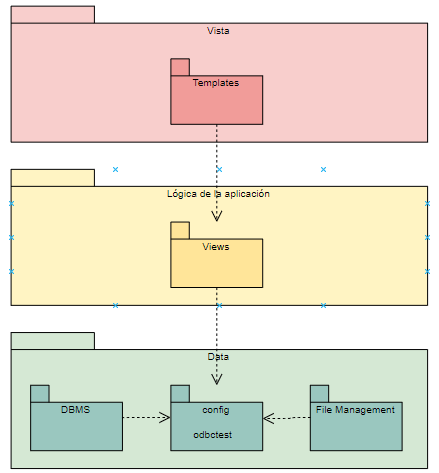
\includegraphics[scale=0.9]{DiagramaPaquetes}\newline

La vista, que es la parte de la interfaz se basa en los templates.\newline
Los templates dependen del fichero views, que es el que controla la lógica y envía los datos a los templates para mostrar unas u otras cosas y permitir distintos accesos por ejemplo.\newline
El views depende de los templates, que le pasan la información que introduce el usuario por pantalla y también depende de los datos recibidos de la base de datos y de los calendarios de Outlook.\newline
Las conexiones con el SGBD y con Outlook, a su vez, dependen del fichero odbctest y config respectivamente para poder establecer la conexión.
